
\documentclass[12pt,onecolumn]{article}
\usepackage[brazilian]{babel}
\usepackage[utf8]{inputenc}
\usepackage{graphicx}
\usepackage{caption}
\usepackage{subcaption}
\usepackage{float}
\usepackage{hyperref}

\begin{document}

\title{Apostila de Gimp}
\author{Renan Teruo Carneiro \\ Wilson Kazuo Mizutani}
\maketitle

\section{Sobre o Gimp}
  O Gimp é legal.

\section{Instalando}
  Baixa e clique avançar-avançar-indução seja feliz.
  Ou sudo apt-get install.

\section{Tutorial}
  Insira motivação aqui.

  \begin{figure}[H]
  \centering
  \begin{subfigure}{.5\textwidth}
    \centering
    
\includegraphics[width=.7\linewidth]{beast-eye.png}
    \label{fig:ex1_before}
  \end{subfigure}%
  \begin{subfigure}{.5\textwidth}
    \centering
    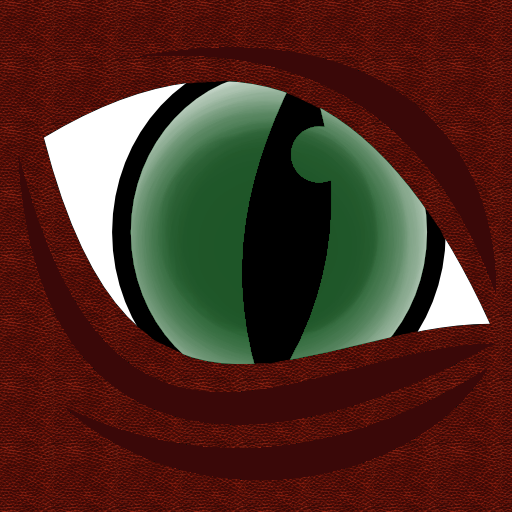
\includegraphics[width=.7\linewidth]{draft00.png}
    \label{fig:ex1_after}
  \end{subfigure}
  \caption{Imagem antes e depois de ter sido editada}
  \label{fig:exercise1}
  \end{figure}

  A imagem original está disponível em (pegue a maior versão possível em PNG)
  \begin{center}
    \url{http://game-icons.net/lorc/original/beast-eye.html}      
  \end{center}

  \subsection{Abrindo a imagem e convertendo para RGBA}
    %% 1) File->Open ou CTRL+O
    %% 2) A imagem fica em grayscale. Vamos criar outra imagem RGBA e passar o
    %%    conteúdo para ela. File->New ou CTRL+N. CTRL+A, CTRL+C, CTR+V.
    \begin{figure}[H]
      \centering
      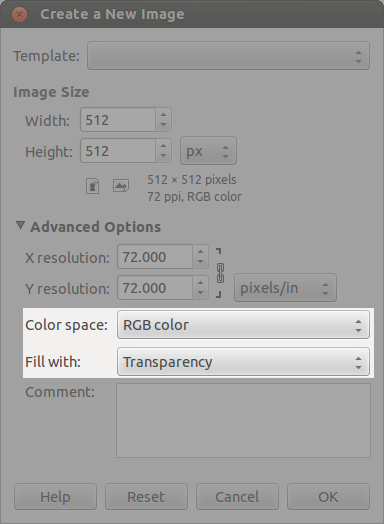
\includegraphics[width=.7\linewidth]{screenshots/00-grayscale_to_RGBA.png}
      \caption{Criando uma imagem RGBA}
      \label{fig:grayscale_to_RGBA}
    \end{figure}
    
  \subsection{Sobre seleções}
    %% 1) Explicação sobre seleções. Só funciona editar se estiver selecionado.
    \begin{figure}[H]
      \centering
      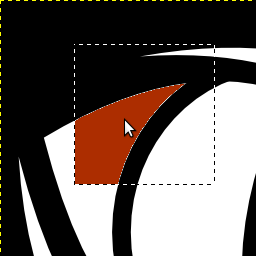
\includegraphics[scale=1]{screenshots/01-selective_painting.png}
      \caption{As ferramentas trabalham apenas nas regiões selecionadas}
      \label{fig:selective_painting}
    \end{figure}
    %% 2) Ferramentas de seleção: retângulo, tesoura e varinha.
    \begin{figure}[H]
      \centering
      \begin{subfigure}{.5\textwidth}
        \centering
        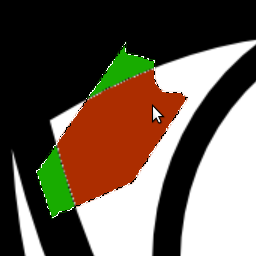
\includegraphics[width=.7\linewidth]{screenshots/02-free_select.png}
        \label{fig:free_select}
      \end{subfigure}%
      \begin{subfigure}{.5\textwidth}
        \centering
        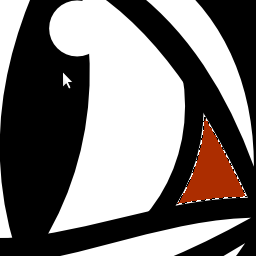
\includegraphics[width=.7\linewidth]{screenshots/03-fuzzy_select.png}
        %\caption{Depois}
        \label{fig:fuzzy_select}
      \end{subfigure}
      \caption{Ferramenta de seleção livre e varinha mágica}
      \label{fig:select_tools}
    \end{figure}
    %% 3) Operações de conjunto: inversão (CTRL+I), conjunção (SHIFT), disjunção
    %%    (CTRL+SHIFT) e diferença (CTRL).
    %% 4) Selecionar o olho e pintar a pupila.
    \begin{figure}[H]
      \centering
      
\includegraphics[width=.5\textwidth]{screenshots/04-pupil.png}
      \caption{Pintamos somente a pupila graças ao funcionamento das seleções}
      \label{fig:pupil}
    \end{figure}
    %% 5) Mencionar como mover seleções.
        
  \subsection{Sobre camadas}
    %% 1) Vamos fazer uma camada para o olho. Selecione apenas o olho.
    %% 2) CTRL+X, CTR+V, colar em nova camada.
    \begin{figure}[H]
      \centering
      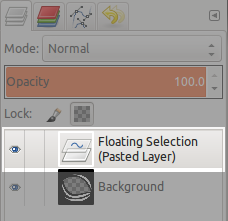
\includegraphics[width=.5\textwidth]{screenshots/05-pasted_layer.png}
      \caption{Seleções coladas ficam em uma camada flutuante}
      \label{fig:pasted_layer}
    \end{figure}
    %% 3) Camadas 101
    %% 4) Renomear camada nova (F2 ou "Edit Layer Attributes")
    %% 5) Redimensionar camada para o tamanho da imagem
    %% 6) Preencher o vazio na camada de baixo (usar balde)
    %% 7) Separar as estrias em outra camada também.
    \begin{figure}[H]
      \centering
      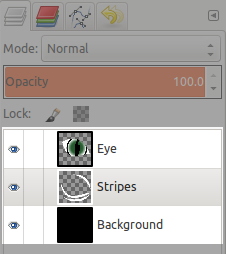
\includegraphics[width=.5\textwidth]{screenshots/07-layers.png}
      \caption{As três camadas no final}
      \label{fig:layers}
    \end{figure}
    
  \subsection{Finalizando}
    %% 1) Pintar as estrias (explicar o modo "fill selection" do balde)
    \begin{figure}[H]
      \centering
      
\includegraphics[width=.5\textwidth]{screenshots/06-partial.png}
      \caption{Resultado quase pronto da edição}
      \label{fig:partial}
    \end{figure}
    %% 2) Preencher o fundo com a textura "Leather" usando balde.
    %% 3) Ajustar cores, tons, etc.
    \begin{figure}[H]
      \centering
      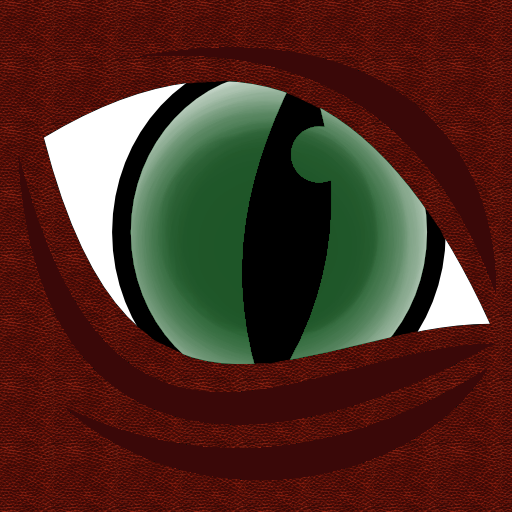
\includegraphics[width=.7\linewidth]{draft00.png}
      \caption{Resultado final}
      \label{fig:final}
    \end{figure}
    %% 4) Proporpupilas melhores.
    
\section{Ferramentas}

  \subsection{Seleção}
    Oi?

  \subsection{Edição}
    É da padaria?
    
  \subsection{Controle de Cor}

\section{Glossário}

\end{document}
